
%(BEGIN_QUESTION)
% Copyright 2009, Tony R. Kuphaldt, released under the Creative Commons Attribution License (v 1.0)
% This means you may do almost anything with this work of mine, so long as you give me proper credit

Determine the process temperature at different times based on the millivolt measurements indicated by the multimeter connected to the thermocouple wires (red to white, black to red) at different locations in the circuit:

$$\includegraphics[width=15.5cm]{i04250x01.eps}$$

\begin{itemize}
\item{} Identify the type of thermocouple used in this process = Type \underbar{\hskip 50pt}
\vskip 5pt
\item{} Measured voltage = 16.101 mV ; meter connected at head ; $T$ = \underbar{\hskip 50pt} deg F
\vskip 5pt
\item{} Measured voltage = $-4.843$ mV ; meter connected at head ; $T$ = \underbar{\hskip 50pt} deg F
\vskip 5pt
\item{} Measured voltage = 7.384 mV ; meter connected at transmitter ; $T$ = \underbar{\hskip 50pt} deg F
\vskip 5pt
\item{} Measured voltage = 15.882 mV ; meter connected at transmitter ; $T$ = \underbar{\hskip 50pt} deg F
\end{itemize}

\underbar{file i04250}
%(END_QUESTION)





%(BEGIN_ANSWER)

\begin{itemize}
\item{} Identify the type of thermocouple used in this process = Type {\bf J}
\item{} Measured voltage = 16.101 mV ; meter connected at head ; $T$ = {\bf 620 to 621} deg F
\item{} Measured voltage = $-4.843$ mV ; meter connected at head ; $T$ = {\bf $-85$ to $-86$} deg F
\item{} Measured voltage = 7.384 mV ; meter connected at transmitter ; $T$ = {\bf 317 to 318} deg F
\item{} Measured voltage = 15.882 mV ; meter connected at transmitter ; $T$ = {\bf 593 to 594} deg F
\end{itemize}

2 points for each correct answer.

%(END_ANSWER)





%(BEGIN_NOTES)

Students will need a type J thermocouple table, referenced in degrees F.

\vskip 10pt

{\bf This question is intended for exams only and not worksheets!}.

%(END_NOTES)


